\chapter{System Design}

\section{Overview}
In this section, we will illustrate the entire system in detail. We will go through all the various technologies that were finalized from the technical review, where they are located in the project structure and what role they have in creating a fluid and realistic experience for the user. In Figure~\ref{image:SystemArch} we can see the high-level design of the project. Each component has a major roll to play in creating this fluid experience and we will discuss how they where implemented now in detail.

\begin{figure}[h!]
	\caption{System Architecture.}
	\label{image:SystemArch}
	\centering
	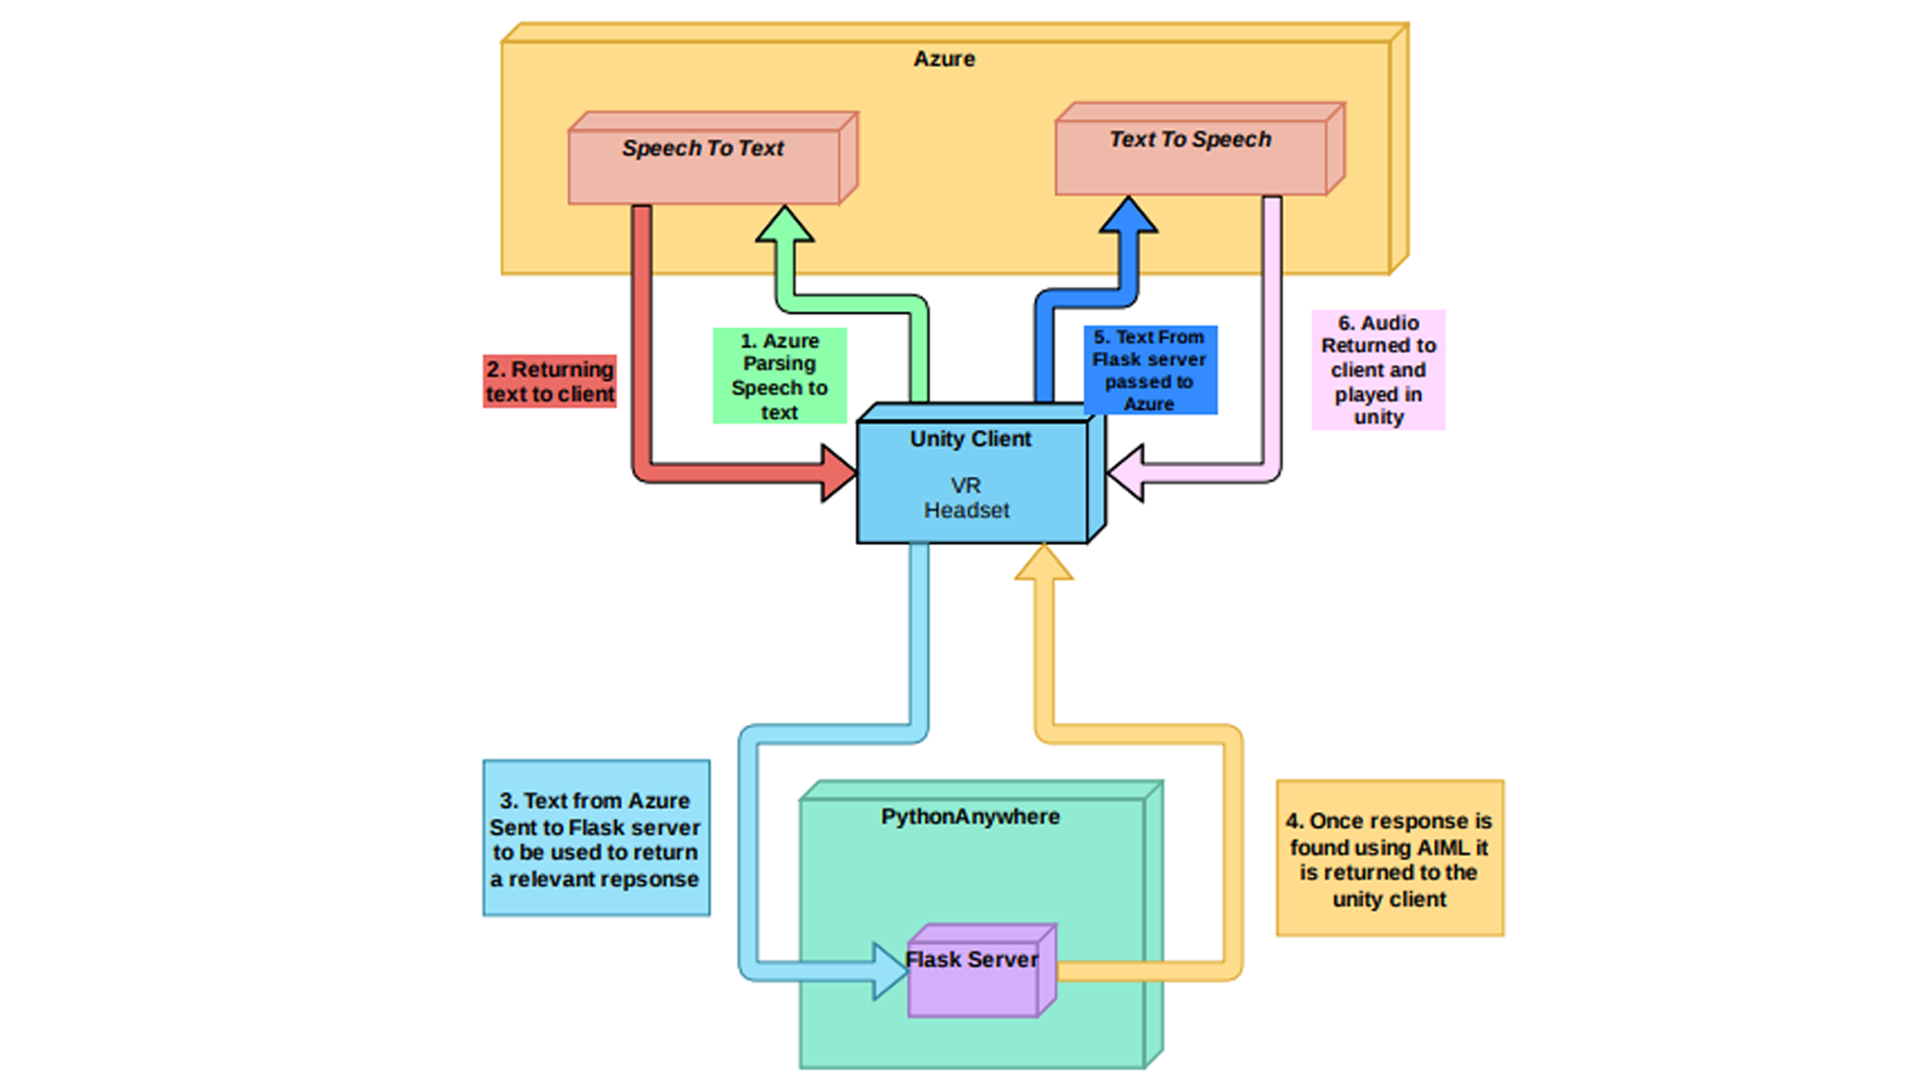
\includegraphics[width=1\textwidth]{Images/uml2.png}
\end{figure}

\section{Unity}
As seen in Figure~\ref{image:SystemArch} Unity is the central component in this application. It is the part that the user interacts with and the part where all the data flows in and out of. Having said that, in this section we will discuss the more graphical side of the implementation and how we did that.

\subsection{3D Models}
Generating realistic bots with realistic models was a problem that was easily solved with the aid of a website called "http://mixamo.com/". This website has an plethora of high quality 3d character models along with animations. Once the model was imported into Unity all that was left to do was give these bots a session ID,random voice, gender based on that voice and a random persona e.g Polite,neutral and rude. These personas would aid us later in deciding which AIML file to use server-side. As seen in the below code snippet this is how we generate all these traits. The session ID is a random number between 1 and 10000. The persona is a integer between zero and three, each number meaning a different persona: 

\begin{table}[!ht]
    \centering
\begin{tabular}{ |p{3cm}|p{5cm}|  }
\hline
\multicolumn{2}{|c|}{NPC Personas} \\
\hline
Number & Persona \\
\hline
0 & Rude NPC \\
\hline
1 & Neutral NPC \\
\hline
2 & Polite NPC \\
\hline

\end{tabular}
    \caption{Personas}
    \label{tab:my_label}
\end{table}


\begin{lstlisting}[language=python]
    public void SetSessionId()
    {
        sessionId = UnityEngine.Random.Range(1, 10000);
    }
    public void SetPersona()
    {
        persona = UnityEngine.Random.Range(0, 3);
    }
    public void SetVoice()
    {
        //0 = male 1= female
        int gender = UnityEngine.Random.Range(0, 2);
        Debug.Log("GENDER:" + gender);
        string[] voicesMale = {"en-US-GuyNeural", "en-IE-Sean"};
        string[] voicesFemale = { "en-US-JessaNeural", "de-DE-KatjaNeural" };
        if (gender == 0)
        {
            int rand = UnityEngine.Random.Range(0, voicesMale.Length);
            voiceName = voicesMale[rand];
        }
        else if(gender == 1)
        {
            int rand = UnityEngine.Random.Range(0, voicesFemale.Length);
            voiceName = voicesFemale[rand];
        }
    }
\end{lstlisting}

Once these traits have been generated all that is left to be done is to generate them in the virtual 3D enviroment. The solution to this can be seen in the below snippet.
This snippet is also wrapped in a for loop to generate multiple random NPCs. There is an array of manually place GameObjects in the virtual world. These GameObjects act as spawning points for a single NPC. Based on the NPCs voice a Male or Female model is loaded then it is spawned in the position and rotation of one of the spawn points according to the index of the loop. After this process is complete we see NPCs standing in all the spawn points. This is how all the NPCs/Bots are spawned in the application.\newline

\begin{lstlisting}[language=python]
    if (copy.GetComponent<NPC>().GetVoiceName() == "en-US-JessaNeural" || copy.GetComponent<NPC>().GetVoiceName() == "de-DE-KatjaNeural")
    {
        int rand = UnityEngine.Random.Range(0, 2);

        if(rand == 0)
        {
            copy = Instantiate(npc2, new Vector3(NPCSpawners[i].position.x, NPCSpawners[i].position.y, NPCSpawners[i].position.z), Quaternion.Euler(0, NPCSpawners[i].rotation.eulerAngles.y, 0));
            copy.GetComponent<NPC>().SetVoice(npcVoice);
            copy.transform.parent = container.transform;
        }else if(rand == 1)
        {
            copy = Instantiate(npc3, new Vector3(NPCSpawners[i].position.x, NPCSpawners[i].position.y, NPCSpawners[i].position.z), Quaternion.Euler(0, NPCSpawners[i].rotation.eulerAngles.y, 0));
            copy.GetComponent<NPC>().SetVoice(npcVoice);
            copy.transform.parent = container.transform;
        }
    }
    else
    {
        copy = Instantiate(npc1, new Vector3(NPCSpawners[i].position.x, NPCSpawners[i].position.y, NPCSpawners[i].position.z), Quaternion.Euler(0, NPCSpawners[i].rotation.eulerAngles.y, 0));
        copy.GetComponent<NPC>().SetVoice(npcVoice);
        copy.transform.parent = container.transform;
    }
\end{lstlisting}


\subsection{Animation}
Animations in our opinion were important in this application. We needed the user to feel as if they were speaking to a person. If the NPCs where static it would have ruined the realism, completely disconnecting the user from this virtual world. As mentioned earlier, we were fortunate to find a website called Mixamo. As well as realistic models it also had animations to go along side them. The process of applying the animation to the model is simple but tedious. Firstly you must add a Animator component to the model/NPC this allows you to manage your animation clips. Once this is done, animations can be added to the animator using a graph-like interface as seen in Figure~\ref{fig:anim}. Each animation is considered as a stater. If certain parameters are met you can change the state, therefore changing the animation.

\begin{figure}[!ht]
    \centering
    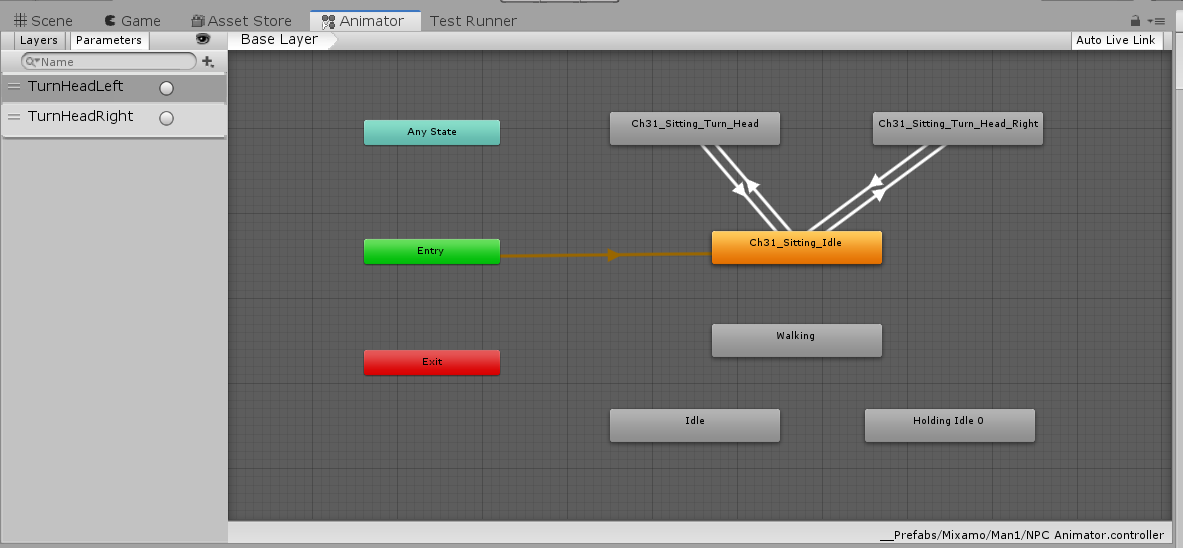
\includegraphics[width=1\textwidth]{Images/animator.PNG}
    \caption{Animator}
    \label{fig:anim}
\end{figure}

\section{HTTP}
In order to communicate with our Flask server we used HTTP. We did so using the UnityEngine.Networking library. Before sending the data we created an object to store the session ID, persona and the user input from the STT service. Once this object was created it was converted to a JSON string. Then this string of json was sent, as seen in the code snippet below, to the Flask server hosted on PythonAnywhere to be processed and return a predicted response from the bot. That response is then sent to the TTS service.

\begin{lstlisting}[language=python]
        string json = new Utilities().ToJsonString(request);
        UnityWebRequest www = UnityWebRequest.Put("http://aaronchannon1.pythonanywhere.com/request", json);
        www.SetRequestHeader("Content-Type", "application/json");
        yield return www.SendWebRequest();

        if (www.isNetworkError || www.isHttpError)
        {
            Debug.Log(www.error);
        }
        else
        {
            string reponse = www.downloadHandler.text;

            try
            {
                string[] reponses = reponse.Split('=');

                TextToSpeech.Instance.ConvertTextToSpeech(reponses[0], voiceName, false);

                new ScoreManager(request.sessionId, Int32.Parse(reponses[1]), request.userInput, reponses[0]).UpdateScore();
            }
            catch
            { 
                TextToSpeech.Instance.ConvertTextToSpeech(reponse, voiceName, false);
            }
        }
\end{lstlisting}

\section{Azure}
\subsection{Azure Speech-to-Text}
%collide with bot
\subsection{Azure Text-to-Speech}

\section{Oculus Quest}

\section{AIML}
% NEED THIS LATER
\begin{figure}[!h]
    \centering
    \begin{lstlisting}[language=PYTHON]
@app.route('/request', methods=['POST'])
def predictResponse():
    # Get json from request.
    sessionId = request.get_json()['sessionId']
    persona = request.get_json()['persona']
    userInput = request.get_json()['userInput']
    print(sessionId)
    print(persona)
    print(userInput)

    # Load specific aiml file depending on persona.
    kernel.respond("load aiml " + str(persona))

    print("DATA:")
    print(kernel.getPredicate("usersName", sessionId))

    # Predict reponse for specific session using user input.
    response = kernel.respond(userInput, sessionId)
    print(response)

    return response

\end{lstlisting}
    \caption{Caption}
    \label{fig:my_label}
\end{figure}


\section{Flask}

\section{PythonAnywhere}
After creating an account the steps to hosting a flask server on PythonAnywhere pretty tedious. Especially if you did not create the Flask server from scratch on the site.

\begin{itemize}
    \item Firstly, you create a web app. This will generate all the necessary files you need to start.
    \item Then we added all our server files to the web app fold that was generated.
    \item Unfortunately, we had not developed the flask server on PythonAnywhere from being so we had to install all the extra libraries at once before we could even get a simple get request working. To install the relevant libraries we had to open a bash constole and pip3.7 install --user "LIB-NAME" every import we had.
    \item Then you must added every import to the WSGI config file.
\end{itemize}
After all this everything worked flawlessly and we were able to get predictions from the Flask server.

\section{MongoDB}